\documentclass[11pt]{article}

\usepackage{geometry}
\usepackage{amsmath,amsthm,amssymb}
\usepackage[table]{xcolor}
\usepackage{fullpage}
\usepackage{enumitem}
\usepackage{tikz-cd}
\usepackage{setspace}
\usepackage{centernot}
\usepackage{graphicx}

\setlength{\parindent}{0.0in}    
\setlength{\parskip}{12pt}

\newtheorem{Thm}{Theorem}[section]
\newtheorem{Lem}[Thm]{Lemma}
\newtheorem{Prop}[Thm]{Proposition}
\newtheorem{Cor}[Thm]{Corollary}
\newtheorem{Rem}[Thm]{Remark}
\newtheorem{Def}[Thm]{Definition}

\begin{document}
\begin{center}
{\LARGE\textbf{COMP4211 - Machine Learning}}
\\{\large{Fall 2024, HKUST}}\\\vspace{1cm}
{\LARGE \textbf {Problem Set}}\\%%%Change the HW Number%%%
\vspace{1cm}

\large \textbf{Name:}
\underline{
Shawn Darren S. Chua
}
\hfill 
\textbf{Student ID:} 
\underline{
20946705
}

\noindent\rule{12cm}{0.4pt}
\end{center}

\textbf{Problem 1.}
\begin{enumerate}[label=(\arabic*)]
\item %1a
\( \\ \)
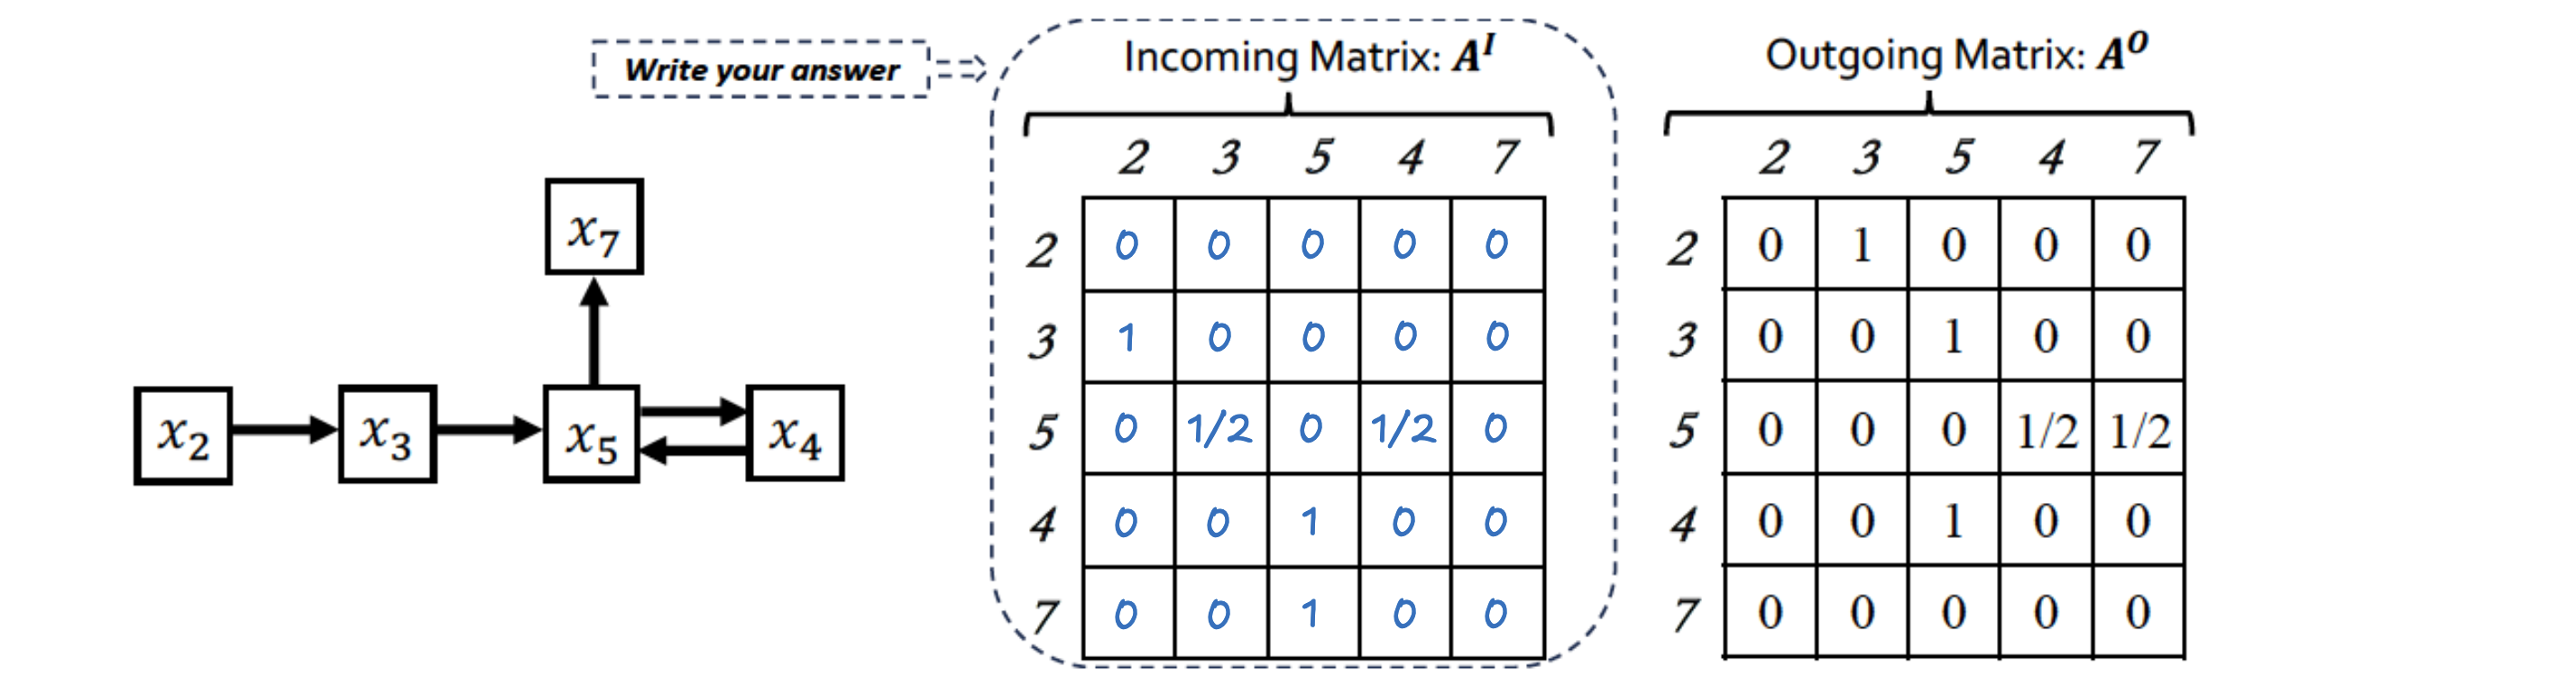
\includegraphics[width=\textwidth]{1a.png}
\( \\ \)

\item %1b
\(h^{l-1^\top}\in \mathbb{R}^d\) and \(h^{l-1^\top}\mathbf{W}^I\in \mathbb{R}^d\), so \(\mathbf{W}^I \in\mathbb{R}^{d\times d}\)

\(h^{l-1^\top}\in \mathbb{R}^d\) and \(h^{l-1^\top}\mathbf{W}^O\in \mathbb{R}^d\), so \(\mathbf{W}^O \in\mathbb{R}^{d\times d}\)

Thus \(\mathbf{W}^I, \mathbf{W}^O\) both have \(d^2\) parameters.
\( \\ \)


\item %1c
\(a_i^l\in\mathbb{R}^{2d\times 1}\) and \(\mathbf{W}_z a_i^l\in\mathbb{R}^{d\times 1}\), so \(\mathbf{W}_z\in\mathbb{R}^{d\times 2d}\)

\(a_i^l\in\mathbb{R}^{2d\times 1}\) and \(\mathbf{W}_r a_i^l\in\mathbb{R}^{d\times 1}\), so \(\mathbf{W}_r\in\mathbb{R}^{d\times 2d}\)

\(a_i^l\in\mathbb{R}^{2d\times 1}\) and \(\mathbf{W}_h a_i^l\in\mathbb{R}^{d\times 1}\), so \(\mathbf{W}_h\in\mathbb{R}^{d\times 2d}\)

Thus \(\mathbf{W}_z, \mathbf{W}_r, \mathbf{W}_h\) all have \(2d^2\) parameters.

\(h_i^{l-1}\in\mathbb{R}^{d\times 1}\) and \(\mathbf{U}_z h_i^{l-1}\in\mathbb{R}^{d\times 1}\), so \(\mathbf{W}_z\in\mathbb{R}^{d\times d}\)

\(h_i^{l-1}\in\mathbb{R}^{d\times 1}\) and \(\mathbf{U}_r h_i^{l-1}\in\mathbb{R}^{d\times 1}\), so \(\mathbf{W}_r\in\mathbb{R}^{d\times d}\)

\(r_i^l \odot h_i^{l-1}\in\mathbb{R}^{d\times 1}\) and \(\mathbf{U}_h \left (r_i^l \odot h_i^{l-1} \right )\in\mathbb{R}^{d\times 1}\), so \(\mathbf{W}_h\in\mathbb{R}^{d\times d}\)

Thus \(\mathbf{U}_z, \mathbf{U}_r, \mathbf{U}_h\) all have \(d^2\) parameters.
\( \\ \)


\item %1d

\( \\ \)


\item %1e
\(\mathbf{W}^I, \mathbf{W}^O\) have a total of \(2d^2\) parameters.

\(\mathbf{b}^I, \mathbf{b}^O\in\mathbb{R}^d\) have a total of \(2d\) parameters.

\(\mathbf{W}_z, \mathbf{W}_r, \mathbf{W}_h\) have a total of \(6d^2\) parameters.

\(\mathbf{U}_z, \mathbf{U}_r, \mathbf{U}_h\) have a total of \(3d^2\) parameters.

\(\mathbf{W}_{q1}, \mathbf{W}_{q2}\) have the same shapes as \(\mathbf{W}_{k1}, \mathbf{W}_{k2}\), so they have a total of \(6d^2\) parameters.

Summing these up, we get \(2d^2 + 2d + 6d^2 + 3d^2 + 6d^2 = 17d^2 + 2d = 170200\) parameters.

\end{enumerate}
\pagebreak
\textbf{Problem 2.}
\begin{enumerate}[label=(\alph*)]
\item %2a


\item %2b


\end{enumerate}
\pagebreak
\end{document}